\documentclass[11pt,a4paper]{report}
\usepackage[textwidth=37em,vmargin=30mm]{geometry}
\usepackage{calc,xunicode,amsmath,amssymb,paralist,enumitem,tabu,booktabs,datetime2,xeCJK,xeCJKfntef,listings}
\usepackage{tocloft,fancyhdr,tcolorbox,xcolor,graphicx,eso-pic,xltxtra,xelatexemoji}

\newcommand{\envyear}[0]{2025}
\newcommand{\envdatestr}[0]{2025-06-27}
\newcommand{\envfinaldir}[0]{webdb/2025/20250627/final}

\usepackage[hidelinks]{hyperref}
\hypersetup{
    colorlinks=false,
    pdfpagemode=FullScreen,
    pdftitle={Web Digest - \envdatestr}
}

\setlength{\cftbeforechapskip}{10pt}
\renewcommand{\cftchapfont}{\rmfamily\bfseries\large\raggedright}
\setlength{\cftbeforesecskip}{2pt}
\renewcommand{\cftsecfont}{\sffamily\small\raggedright}

\setdefaultleftmargin{2em}{2em}{1em}{1em}{1em}{1em}

\usepackage{xeCJK,xeCJKfntef}
\xeCJKsetup{PunctStyle=plain,RubberPunctSkip=false,CJKglue=\strut\hskip 0pt plus 0.1em minus 0.05em,CJKecglue=\strut\hskip 0.22em plus 0.2em}
\XeTeXlinebreaklocale "zh"
\XeTeXlinebreakskip = 0pt


\setmainfont{Brygada 1918}
\setromanfont{Brygada 1918}
\setsansfont{IBM Plex Sans}
\setmonofont{JetBrains Mono NL}
\setCJKmainfont{Noto Serif CJK SC}
\setCJKromanfont{Noto Serif CJK SC}
\setCJKsansfont{Noto Sans CJK SC}
\setCJKmonofont{Noto Sans CJK SC}

\setlength{\parindent}{0pt}
\setlength{\parskip}{8pt}
\linespread{1.15}

\lstset{
	basicstyle=\ttfamily\footnotesize,
	numbersep=5pt,
	backgroundcolor=\color{black!5},
	showspaces=false,
	showstringspaces=false,
	showtabs=false,
	tabsize=2,
	captionpos=b,
	breaklines=true,
	breakatwhitespace=true,
	breakautoindent=true,
	linewidth=\textwidth
}






\newcommand{\coverpic}[2]{
    % argv: itemurl, authorname
    Cover photo by #2~~(\href{#1}{#1})
}
\newcommand{\makeheader}[0]{
    \begin{titlepage}
        % \newgeometry{hmargin=15mm,tmargin=21mm,bmargin=12mm}
        \begin{center}
            
            \rmfamily\scshape
            \fontspec{BaskervilleF}
            \fontspec{Old Standard}
            \fontsize{59pt}{70pt}\selectfont
            WEB\hfill DIGEST
            
            \vfill
            % \vskip 30pt
            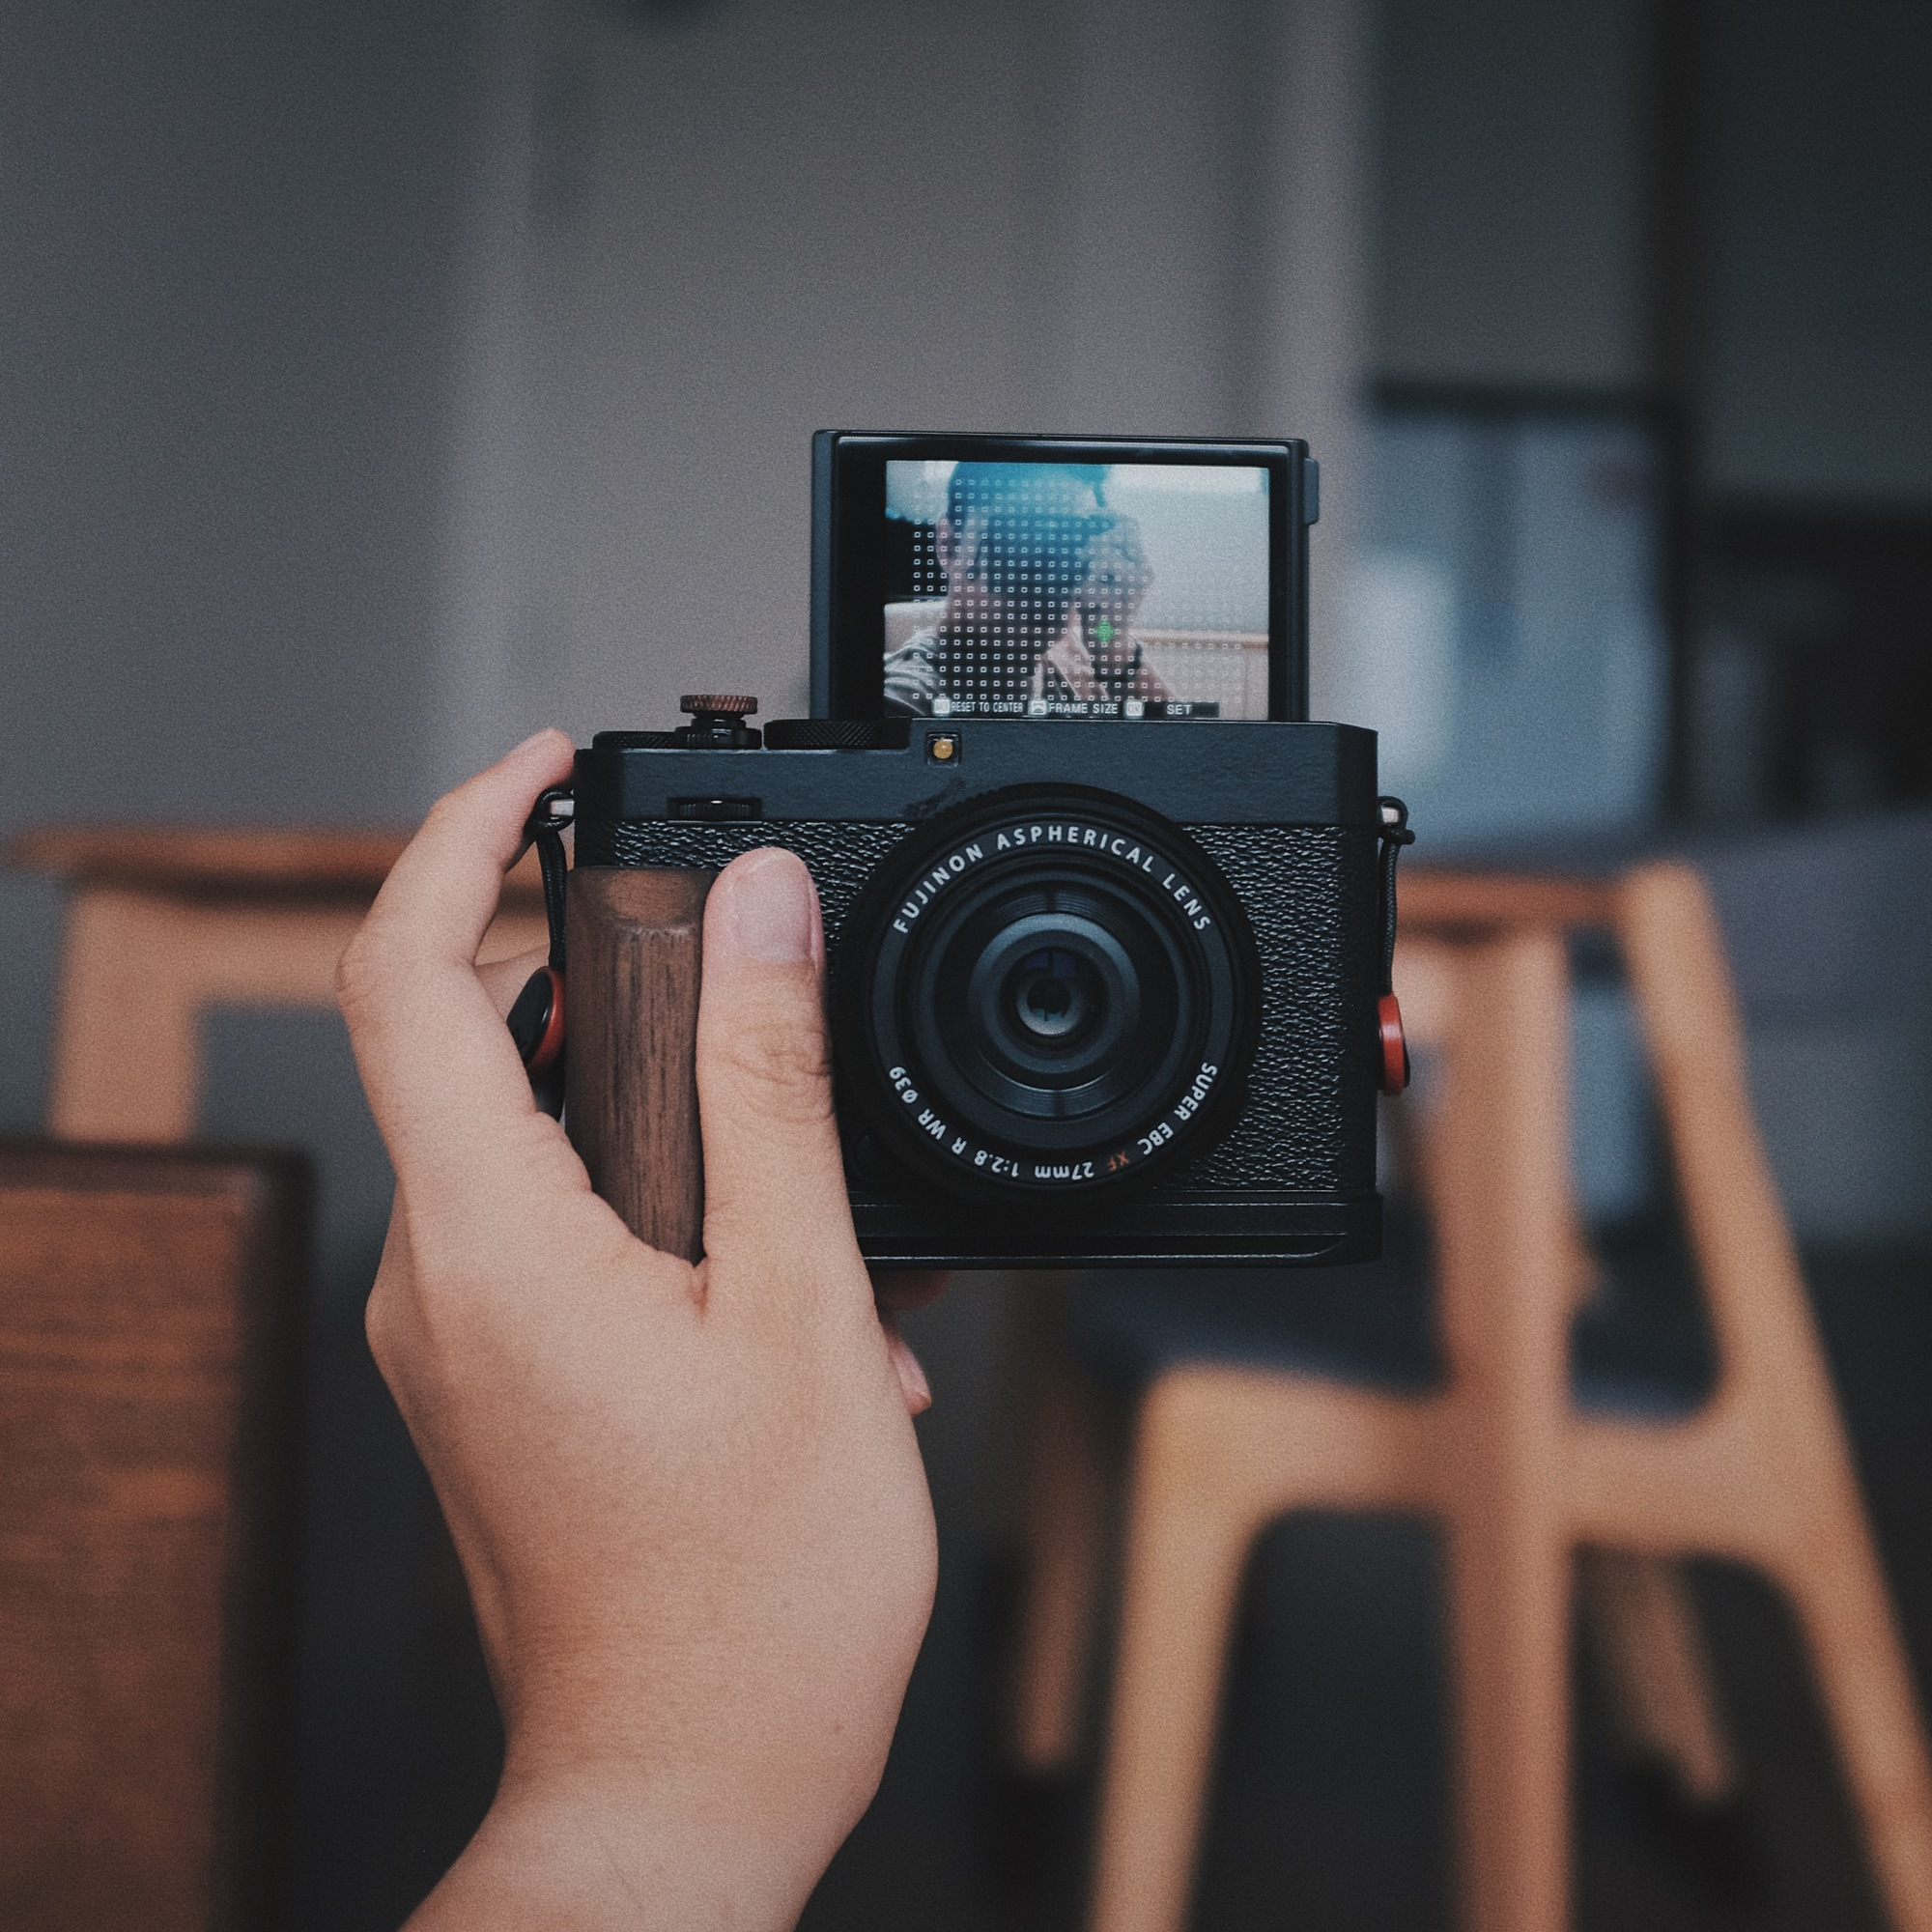
\includegraphics[width=\linewidth]{\envfinaldir/coverpic-prod.jpg}\par
            % \vskip 30pt
            \vfill

            \normalsize\rmfamily\scshape
            \copyright{} The Web Digest Project \hfill\large \envdatestr
        \end{center}
    \end{titlepage}
    % \restoregeometry
}
\newcommand{\simplehref}[1]{%
    \textcolor{blue!80!green}{\href{#1}{#1}}%
}
\renewcommand{\contentsname}{\center\Huge\sffamily\bfseries Contents\par\vskip 20pt}
\newcounter{ipartcounter}
\setcounter{ipartcounter}{0}
\newcommand{\ipart}[1]{
    % \vskip 20pt
    \clearpage
    \stepcounter{ipartcounter}
    \phantomsection
    \addcontentsline{toc}{chapter}{#1}
    % \begin{center}
    %     \Huge
    %     \sffamily\bfseries
    %     #1
    % \end{center}
    % \vskip 20pt plus 7pt
}
\newcounter{ichaptercounter}
\setcounter{ichaptercounter}{0}
\newcommand{\ichapter}[1]{
    % \vskip 20pt
    \clearpage
    \stepcounter{ichaptercounter}
    \phantomsection
    \addcontentsline{toc}{section}{\numberline{\arabic{ichaptercounter}}#1}
    \begin{center}
        \Huge
        \sffamily\bfseries
        #1
    \end{center}
    \vskip 20pt plus 7pt
}
\newcommand{\entrytitlefont}[1]{\subsection*{\raggedright\Large\sffamily\bfseries#1}}
\newcommand{\entryitemGeneric}[2]{
    % argv: title, url
    \parbox{\linewidth}{
        \entrytitlefont{#1}\par\vskip 5pt
        \footnotesize\ttfamily\mdseries
        \simplehref{#2}
    }\vskip 11pt plus 11pt minus 1pt
}
\newcommand{\entryitemGithub}[3]{
    % argv: title, url, desc
    \parbox{\linewidth}{
        \entrytitlefont{#1}\par\vskip 5pt
        \footnotesize\ttfamily\mdseries
        \simplehref{#2}\par\vskip 5pt
        \small\rmfamily\mdseries#3
    }\vskip 11pt plus 11pt minus 1pt
}
\newcommand{\entryitemAp}[3]{
    % argv: title, url, desc
    \parbox{\linewidth}{
        \entrytitlefont{#1}\par\vskip 5pt
        \footnotesize\ttfamily\mdseries
        \simplehref{#2}\par\vskip 5pt
        \small\rmfamily\mdseries#3
    }\vskip 11pt plus 11pt minus 1pt
}
\newcommand{\entryitemHackernews}[3]{
    % argv: title, hnurl, rawurl
    % \parbox{\linewidth}{
    %     \entrytitlefont{#1}\par\vskip 5pt
    %     \footnotesize\ttfamily\mdseries
    %     \simplehref{#3}\par
    %     \textcolor{black!50}{\href{#2}{#2}}
    % }\vskip 11pt plus 11pt minus 1pt
    \begin{minipage}{\linewidth}
            \entrytitlefont{#1}\par\vskip 5pt
            \footnotesize\ttfamily\mdseries
            \simplehref{#3}\par
            \textcolor{black!50}{\href{#2}{#2}}
    \end{minipage}\par\vskip 11pt plus 11pt minus 1pt
}







\begin{document}

\makeheader

\tableofcontents\clearpage




\ipart{Developers}
\ichapter{Hacker News}
\entryitemTwoLinks{Matrix v1.15}{https://news.ycombinator.com/item?id=44390740}{https://matrix.org/blog/2025/06/26/matrix-v1.15-release/}

\entryitemTwoLinks{AI Is Dehumanization Technology}{https://news.ycombinator.com/item?id=44390576}{https://thedabbler.patatas.ca/pages/ai-is-dehumanization-technology.html}

\entryitemTwoLinks{"Why is the Rust compiler so slow?"}{https://news.ycombinator.com/item?id=44390488}{https://sharnoff.io/blog/why-rust-compiler-slow}

\entryitemTwoLinks{US economy shrank 0.5\% in the first quarter, worse than earlier estimates}{https://news.ycombinator.com/item?id=44390454}{https://apnews.com/article/economy-tariffs-trump-gdp-shrink-86d1f15e66c646ac4ce88ffc0a956942}

\entryitemTwoLinks{Introducing Gemma 3n}{https://news.ycombinator.com/item?id=44389202}{https://developers.googleblog.com/en/introducing-gemma-3n-developer-guide/}

\entryitemTwoLinks{FLUX.1 Kontext [Dev] – Open Weights for Image Editing}{https://news.ycombinator.com/item?id=44388387}{https://bfl.ai/announcements/flux-1-kontext-dev}

\entryitemTwoLinks{Show HN: I built an AI dataset generator}{https://news.ycombinator.com/item?id=44388093}{https://github.com/metabase/dataset-generator}

\entryitemTwoLinks{Launch HN: Issen (YC F24) – Personal AI language tutor}{https://news.ycombinator.com/item?id=44387828}{https://news.ycombinator.com/item?id=44387828}

\entryitemTwoLinks{AlphaGenome: AI for better understanding the genome}{https://news.ycombinator.com/item?id=44387659}{https://deepmind.google/discover/blog/alphagenome-ai-for-better-understanding-the-genome/}

\entryitemTwoLinks{Learnings from building AI agents}{https://news.ycombinator.com/item?id=44386887}{https://www.cubic.dev/blog/learnings-from-building-ai-agents}

\entryitemTwoLinks{I fought in Ukraine and here's why FPV drones kind of suck}{https://news.ycombinator.com/item?id=44385892}{https://warontherocks.com/2025/06/i-fought-in-ukraine-and-heres-why-fpv-drones-kind-of-suck/}

\entryitemTwoLinks{Apptainer: Application Containers for Linux}{https://news.ycombinator.com/item?id=44385742}{https://apptainer.org/}

\entryitemTwoLinks{The first non-opoid painkiller}{https://news.ycombinator.com/item?id=44385612}{https://www.worksinprogress.news/p/the-first-non-opioid-painkiller}

\entryitemTwoLinks{Snow - Classic Macintosh emulator}{https://news.ycombinator.com/item?id=44385562}{https://snowemu.com/}

\entryitemTwoLinks{LLM code generation may lead to an erosion of trust}{https://news.ycombinator.com/item?id=44384610}{https://jaysthoughts.com/aithoughts1}

\entryitemTwoLinks{Puerto Rico's Solar Microgrids Beat Blackout}{https://news.ycombinator.com/item?id=44382834}{https://spectrum.ieee.org/puerto-rico-solar-microgrids}

\entryitemTwoLinks{Define policy forbidding use of AI code generators}{https://news.ycombinator.com/item?id=44382752}{https://github.com/qemu/qemu/commit/3d40db0efc22520fa6c399cf73960dced423b048}

\entryitemTwoLinks{The Hollow Men of Hims}{https://news.ycombinator.com/item?id=44382582}{https://www.alexkesin.com/p/the-hollow-men-of-hims}

\entryitemTwoLinks{Microsoft Dependency Has Risks}{https://news.ycombinator.com/item?id=44381358}{https://blog.miloslavhomer.cz/p/microsoft-dependency-has-risks}

\entryitemTwoLinks{A new pyramid-like shape always lands the same side up}{https://news.ycombinator.com/item?id=44381297}{https://www.quantamagazine.org/a-new-pyramid-like-shape-always-lands-the-same-side-up-20250625/}


\ipart{Developers~~~~(zh-Hans)}
\ichapter{Solidot}
\entryitemGeneric{\hskip 0pt{}韦伯望远镜可能首次直接获得系外行星影像}{https://www.solidot.org/story?sid=81658}

\entryitemGeneric{\hskip 0pt{}ispace 登月舱登月失败源于高度计}{https://www.solidot.org/story?sid=81657}

\entryitemGeneric{\hskip 0pt{}一次性电子烟毒性大于传统香烟}{https://www.solidot.org/story?sid=81656}

\entryitemGeneric{\hskip 0pt{}法国里昂淘汰微软软件以实现数字主权}{https://www.solidot.org/story?sid=81655}

\entryitemGeneric{\hskip 0pt{}过度捕捞导致鳕鱼体型缩小一半}{https://www.solidot.org/story?sid=81654}

\entryitemGeneric{\hskip 0pt{}Bernie Sanders 认为如果 AI 提高了员工生产力那么应该推行一周四天工作制}{https://www.solidot.org/story?sid=81653}

\entryitemGeneric{\hskip 0pt{}掌机测试发现游戏在 SteamOS 上的性能高于 Windows 11}{https://www.solidot.org/story?sid=81652}

\entryitemGeneric{\hskip 0pt{}Aaron Sorkin 制作《社交网络》续集}{https://www.solidot.org/story?sid=81651}

\entryitemGeneric{\hskip 0pt{}法官裁决 Meta 使用版权书籍训练大模型属于合理使用 }{https://www.solidot.org/story?sid=81650}

\entryitemGeneric{\hskip 0pt{}OpenAI 在企业级市场抢微软的客户}{https://www.solidot.org/story?sid=81649}

\entryitemGeneric{\hskip 0pt{}运送近百辆电动汽车的货船起火沉没}{https://www.solidot.org/story?sid=81648}

\entryitemGeneric{\hskip 0pt{}微软发布编辑器 MS-DOS Editor 的 Rust 版本}{https://www.solidot.org/story?sid=81647}

\entryitemGeneric{\hskip 0pt{}法官裁决 Anthropic 使用书籍训练 AI 是合理使用,但使用盗版书籍训练并不是}{https://www.solidot.org/story?sid=81646}

\entryitemGeneric{\hskip 0pt{}《侏罗纪世界:进化 3》放弃使用生成式 AI}{https://www.solidot.org/story?sid=81645}

\entryitemGeneric{\hskip 0pt{}Anker 等公司召回的移动电源使用了安普瑞斯的电芯 }{https://www.solidot.org/story?sid=81644}

\entryitemGeneric{\hskip 0pt{}微软向 Windows 10 用户提供扩展安全更新}{https://www.solidot.org/story?sid=81643}

\entryitemGeneric{\hskip 0pt{}阳光为什么能高效的蒸发水}{https://www.solidot.org/story?sid=81642}

\entryitemGeneric{\hskip 0pt{}美国众议院禁止工作人员使用 WhatsApp}{https://www.solidot.org/story?sid=81641}

\entryitemGeneric{\hskip 0pt{}Fedora 讨论放弃支持 32 位包}{https://www.solidot.org/story?sid=81640}

\entryitemGeneric{\hskip 0pt{}中国五月份太阳能装机容量创下新记录}{https://www.solidot.org/story?sid=81639}\ichapter{V2EX}
\entryitemGeneric{\hskip 0pt{}[Google] 大家 google voice 号码在哪里买的}{https://www.v2ex.com/t/1141344}

\entryitemGeneric{\hskip 0pt{}[天黑以后] 20250627 午夜俱乐部}{https://www.v2ex.com/t/1141343}

\entryitemGeneric{\hskip 0pt{}[问与答] 电动牙刷有啥靠谱的推荐}{https://www.v2ex.com/t/1141342}

\entryitemGeneric{\hskip 0pt{}[分享创造] vibe coding 做了个科研图库网站,欢迎提建议}{https://www.v2ex.com/t/1141341}

\entryitemGeneric{\hskip 0pt{}[宽带症候群] 特殊宽带套餐汇总帖}{https://www.v2ex.com/t/1141340}

\entryitemGeneric{\hskip 0pt{}[分享创造] 歌词视频生成器}{https://www.v2ex.com/t/1141339}

\entryitemGeneric{\hskip 0pt{}[Apple] 分享一个关于 Magic Keyboard 开关机制的有趣发现}{https://www.v2ex.com/t/1141338}

\entryitemGeneric{\hskip 0pt{}[问与答] 志愿填报寻求建议}{https://www.v2ex.com/t/1141336}

\entryitemGeneric{\hskip 0pt{}[小米] yu7 起售价 25w 三分钟内大定 20w,不是说好的通缩下行吗}{https://www.v2ex.com/t/1141334}

\entryitemGeneric{\hskip 0pt{}[Apple] Apple Passwords 更新 History 功能}{https://www.v2ex.com/t/1141333}

\entryitemGeneric{\hskip 0pt{}[macOS] 小记一下 macOS 26 beta2 暂时不能用的 APP}{https://www.v2ex.com/t/1141332}

\entryitemGeneric{\hskip 0pt{}[问与答] 志愿填报}{https://www.v2ex.com/t/1141331}

\entryitemGeneric{\hskip 0pt{}[生活] 买了个小佩猫砂盆,没想到是``锁区设备''——国产硬件厂商又在重演老路?}{https://www.v2ex.com/t/1141330}

\entryitemGeneric{\hskip 0pt{}[问与答] bootstrap 怎么制作弹出式菜单?}{https://www.v2ex.com/t/1141329}

\entryitemGeneric{\hskip 0pt{}[电动汽车] 小米 YU 7 的座椅为啥不配通风?}{https://www.v2ex.com/t/1141327}

\entryitemGeneric{\hskip 0pt{}[macOS] 突然发现 edge 支持鼠标手势了}{https://www.v2ex.com/t/1141326}

\entryitemGeneric{\hskip 0pt{}[Apple] macOS 15.5,储存空间中的系统数据如何清理?}{https://www.v2ex.com/t/1141325}

\entryitemGeneric{\hskip 0pt{}[全球工单系统] 江苏地区,中国移动有哪些营业厅可以打印 21 年至 23 年的通讯记录}{https://www.v2ex.com/t/1141324}

\entryitemGeneric{\hskip 0pt{}[分享创造] 微信 Markdown 编辑器插件再升级}{https://www.v2ex.com/t/1141323}

\entryitemGeneric{\hskip 0pt{}[程序员] 感觉 claude code 让我成为了技术 leader}{https://www.v2ex.com/t/1141322}

\entryitemGeneric{\hskip 0pt{}[酷工作] 有招聘远程办公 运维的吗?兼职、全职}{https://www.v2ex.com/t/1141321}

\entryitemGeneric{\hskip 0pt{}[Next.js] 发现很多人不了解 Next.js}{https://www.v2ex.com/t/1141320}

\entryitemGeneric{\hskip 0pt{}[问与答] 二本能学计算机专业吗}{https://www.v2ex.com/t/1141317}

\entryitemGeneric{\hskip 0pt{}[酷工作] [杭州]大模型工程师急招}{https://www.v2ex.com/t/1141315}

\entryitemGeneric{\hskip 0pt{}[macOS] appstored 一直在下载数据,大家有什么看法吗?}{https://www.v2ex.com/t/1141314}

\entryitemGeneric{\hskip 0pt{}[嵌入式开发] 个人认为嵌入式领域最无用的发明---色环电阻}{https://www.v2ex.com/t/1141313}

\entryitemGeneric{\hskip 0pt{}[V2EX] 铜币用完了会发生什么}{https://www.v2ex.com/t/1141311}

\entryitemGeneric{\hskip 0pt{}[职场话题] 字节部门了解求助大佬}{https://www.v2ex.com/t/1141310}

\entryitemGeneric{\hskip 0pt{}[程序员] [macos] 发现多台 mac 之间的一个小问题}{https://www.v2ex.com/t/1141309}

\entryitemGeneric{\hskip 0pt{}[宽带症候群] 联通 PCDN 限速}{https://www.v2ex.com/t/1141308}

\entryitemGeneric{\hskip 0pt{}[酷工作] [蚂蚁招聘] 短视频推荐算法工程师}{https://www.v2ex.com/t/1141307}

\entryitemGeneric{\hskip 0pt{}[问与答] 最近想自己做点硬件玩玩,有什么比较基础的套装推荐的吗?}{https://www.v2ex.com/t/1141305}

\entryitemGeneric{\hskip 0pt{}[酷工作] [杭州] [高级 web 前端开发] 自动驾驶(全职)}{https://www.v2ex.com/t/1141304}

\entryitemGeneric{\hskip 0pt{}[分享创造] 查看英文文献,应该有一种英文 碎碎念、伴读 AI 工具}{https://www.v2ex.com/t/1141302}

\entryitemGeneric{\hskip 0pt{}[问与答] 硼酸/硼砂怎么无害化处理?}{https://www.v2ex.com/t/1141300}

\entryitemGeneric{\hskip 0pt{}[程序员] Claude Code 交友群}{https://www.v2ex.com/t/1141299}

\entryitemGeneric{\hskip 0pt{}[程序员] 有没有 AI 可以做一个完整小型项目?}{https://www.v2ex.com/t/1141298}

\entryitemGeneric{\hskip 0pt{}[Apple] MagSafe 外接电池不能上国内飞机了}{https://www.v2ex.com/t/1141297}

\entryitemGeneric{\hskip 0pt{}[分享创造] 我开发了一个免费实用的``家庭菜园种植计划计算器''网站,分享给大家!}{https://www.v2ex.com/t/1141296}

\entryitemGeneric{\hskip 0pt{}[教育] 给 2025 高考生做了一个 AI 专业填报小程序}{https://www.v2ex.com/t/1141293}

\entryitemGeneric{\hskip 0pt{}[美酒与美食] 第一次吃桂味,确实要好吃一点}{https://www.v2ex.com/t/1141291}

\entryitemGeneric{\hskip 0pt{}[云计算] 阿里云 ECS 被释放了 还能找回数据吗}{https://www.v2ex.com/t/1141289}

\entryitemGeneric{\hskip 0pt{}[前端开发] 请教一个大模型生成错误 markdown 内容前端检测的问题}{https://www.v2ex.com/t/1141286}

\entryitemGeneric{\hskip 0pt{}[分享创造] 管理课程体系,从初级管理者经理入门,到中间总监承上启下,到高层高管战略启迪。}{https://www.v2ex.com/t/1141285}

\entryitemGeneric{\hskip 0pt{}[问与答] 想问一下为什么 cursor 的 ssh 有时候会这么慢?}{https://www.v2ex.com/t/1141283}

\entryitemGeneric{\hskip 0pt{}[问与答] 求推荐的户外移动电源}{https://www.v2ex.com/t/1141282}

\entryitemGeneric{\hskip 0pt{}[创业组队] 有网安、渗透方面的大佬吗,这边组团队需要一个真正的这方面的大佬,钱不是问题,有意者联系发简历或者聊聊,一起挣钱!(最好是在西安或者成都)}{https://www.v2ex.com/t/1141281}

\entryitemGeneric{\hskip 0pt{}[Go 编程语言] go run main.go 特别慢}{https://www.v2ex.com/t/1141280}

\entryitemGeneric{\hskip 0pt{}[分享创造] 🎁 [早鸟优惠+送会员] 鸽了又鸽,但这次真的来了!我做的 Mac 屏幕录制软件 ScreenSage Pro 上线,早鸟特惠也终于来了!}{https://www.v2ex.com/t/1141279}

\entryitemGeneric{\hskip 0pt{}[Cursor] 求问 cursor 当前付费方案推荐}{https://www.v2ex.com/t/1141278}


\ipart{Generic News}







\clearpage
\leavevmode\vfill
\footnotesize

Copyright \copyright{} 2023-2025 Neruthes and other contributors.

This document is published with CC BY-NC-ND 4.0 license.

The entries listed in this newsletter may be copyrighted by their respective creators.

This newsletter is generated by the Web Digest project.

The newsletters are also delivered via Telegram channel \CJKunderline{\href{https://t.me/webdigestchannel}{https://t.me/webdigestchannel}}.\\
RSS feed is available at \CJKunderline{\href{https://webdigest.pages.dev/rss.xml}{https://webdigest.pages.dev/rss.xml}}.

This newsletter is available in PDF at
\CJKunderline{\href{https://webdigest.pages.dev/}{https://webdigest.pages.dev/}}.

The source code being used to generate this newsletter is available at\\
\CJKunderline{\href{https://github.com/neruthes/webdigest}{https://github.com/neruthes/webdigest}}.

This newsletter is also available in
\CJKunderline{\href{http://webdigest.pages.dev/readhtml/\envyear/WebDigest-20250627.html}{HTML}} and
\CJKunderline{\href{https://github.com/neruthes/webdigest/blob/master/markdown/\envyear/WebDigest-20250627.md}{Markdown}}.


\coverpic{https://unsplash.com/photos/h9T0dXfqkxU}{Europeana}


\end{document}
